\chapter{Nonlinear Instability for the Periodic Simulation}
\label{c_nlin_periodic}

In this chapter, I use the energy dynamics machinery developed in the last chapter to show where in wavenumber space and to which fields energy is deposited, how it's transferred,
and where it's dissipated. I show that the linear instability plasma paradigm doesn't hold for the LAPD simulations, but rather, a complex nonlinear instability process dominates
the energy dynamics.
Furthermore, in this chapter, I consider only the simulations with periodic boundary conditions: the Periodic simulation and the $n=0$ suppressed simulation. I analyze the remaining simulations
(Dirichlet, Neumann, and Sheath) in the next chapter.


\section{The Energy Spectra}
\label{s_en_spec}

\begin{figure}[!ht]
\centerline{\includegraphics[]{energy_spectra}}
\caption{Energy k-Spectra}
\label{energy_spectra}
\end{figure}

Although I have already discussed the relative importance of the $n=0$ fluctuation flute structures and shown evidence for this in Figs.~\ref{3D_turb_anim},~\ref{rms_evolution}, and
~\ref{n_statistics}, I now use the energy expressions in Eqs.~\ref{ENk},~\ref{Ephik},~\ref{ETk}, and~\ref{Evk} to show a detailed look at the energy
wavenumber spectra. The spectra for the four fields in $(m,n)$ space are shown in Fig.~\ref{energy_spectra}. As expected from Figs.~\ref{3D_turb_anim},~\ref{rms_evolution}, and
~\ref{n_statistics}, most of the density energy $E_N(\vec{k})$ is located at $n=0$ (and $1 < m < 10$). This wavenumber location is much different from my expectation which was
that of the fastest growing linear eigenmode, which is at $(n = 1, m = 60)$. Additionally, $E_T(\vec{k})$ and $E_\phi(\vec{k})$ have similar-looking spectra as $E_N(\vec{k})$, though
the actual magnitudes of the energy are quite different for the three fields. Finally, $E_v(\vec{k})$ has a remarkably different energy spectrum than the other fields. Most of
the energy is contained at $n \ge 1$ and $m \sim 30$, which is somewhat similar to the linear eigenmode growth rate spectrum, though $m$ is lower.

Although these results are rather unexpected given the hypothesis that the most unstable linear eigenmode should pump energy into the turbulent system, one could still build upon this
hypothesis to explain the nature of the spectra. 
In fact, in Ref.~\cite{Umansky2011}, my collaborators and I posited and tested this hypothesis. Our specific hypothesis was that the most unstable linear eigenmode pumped energy into the system at
its characteristic wavenumber and then proceeded to cascade energy forward and backward into other waves. The inverse cascade into $n=0$ would be particularly strong to account for all of
the energy in the $n=0$ Fourier components.

Our test of this inverse cascade revolved around the use of a particular bicoherence three wave interaction, namely that between
three density fluctuation Fourier modes of $(n,m)=(1,25),(-1,-24)$ and $(0,1)$. Note that in that study, we used a different set of profiles and parameters for the simulation 
than the one I use in this report, and the dominant azimuthal mode numbers in that study were smaller than those in this report.
In any case, in Ref.~\cite{Umansky2011}, we found a strong bicoherence amplitude for this three-wave interaction
and assumed that this meant that the waves with $(n,m)=(1,25)$ and $(-1,-24)$ coupled to transfer their energy
to waves with $(0,1)$. This fit within the standard linear instability paradigm because linear eigenmodes with $(n,m) \sim (\pm 1, \pm 25)$ were the most unstable for that system.
Unfortunately, bicoherence is only a vague proxy for three-wave energy interaction, and it doesn't indicate a direction of energy transfer. 
As I later worked on energy dynamics calculations, I discovered, to my surprise, that we had the direction of energy transfer backwards! 
Our assumption regarding the direction of energy transfer was wrong. The paradigmatic plasma turbulence view led us astray.


\section{Energy Dynamics Results}
\label{s_per_en_dyn}

\subsection{Dynamics Details}
\label{ss_dyn_details}


\begin{figure}[!ht]
\centerline{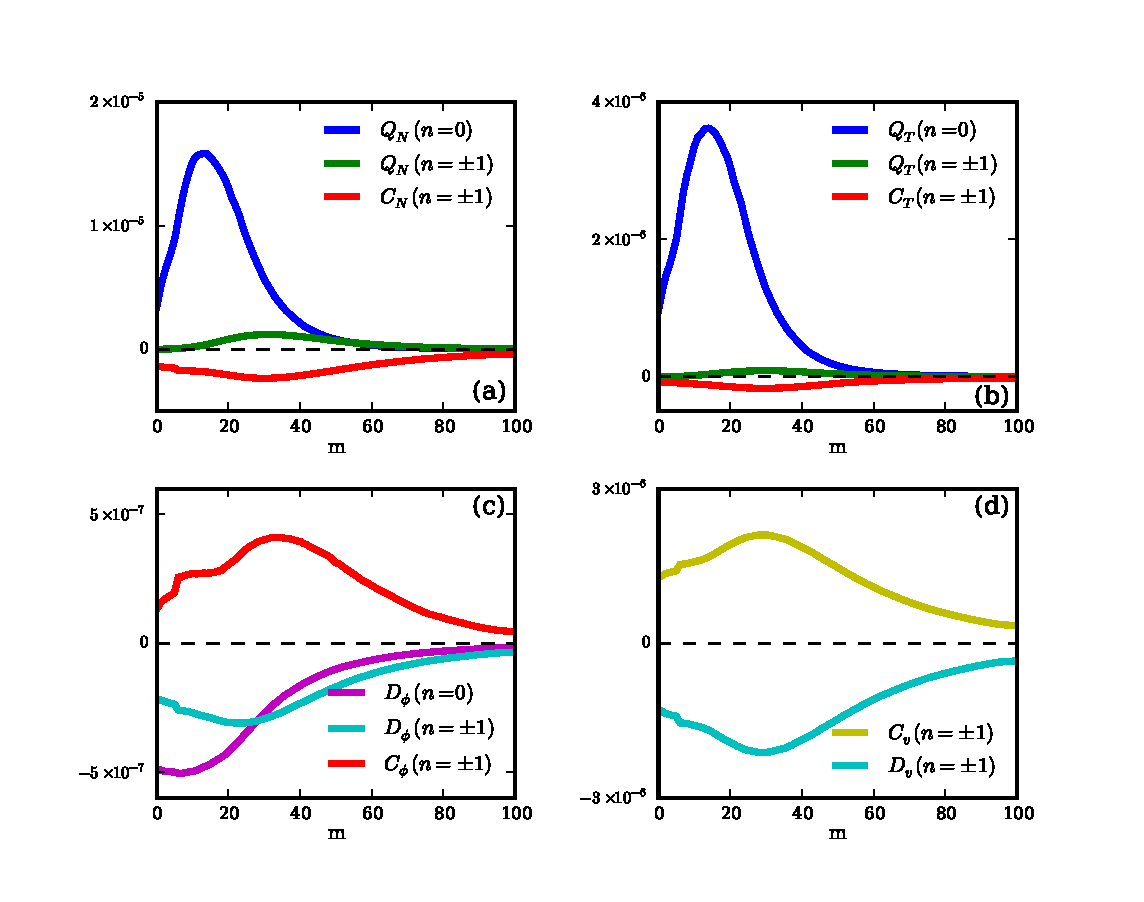
\includegraphics[]{mn_dynamics}}
\caption{Periodic simulation energy dynamics}
\label{mn_dynamics}
\end{figure}


The full energy dynamics analysis using the machinery of Chapter~\ref{c_en_formalism} removes any ambiguity regarding the locations and magnitudes of energy injection into the fluctuations
and direction of energy transfer between different Fourier modes. In fact, the full dynamics contains so much information that it can be difficult to digest it all. I therefore try to
focus on the most important parts, especially those that are crucial to the nonlinear instability. First, in Fig.~\ref{mn_dynamics}, I show values for some of the $Q_j, C_j,$ and $D_j$
terms in the energy dynamics equations for $n=0, \pm 1$ and $0 \le m \le 100$,
neglecting all dynamics with $|n| \ge 2$, which have relatively small values and are mostly insignificant. The dynamics curves are all averaged over a time period during the
turbulent stage of the simulation where the dynamics processes have all reached a quasi-steady state.
The label $n = \pm 1$ represents the addition of terms with $n=1$ and $n=-1$.
Fig.~\ref{mn_dynamics} a) reveals the density potential energy injection ($Q_N$) and the adiabatic response transfer ($C_N$). I don't show the dissipation ($D_N$) in this figure, which
is why the curves don't seem to add up to zero as they would if all dynamics were shown.
Nevertheless, this figure immediately reveals that the majority of the energy is injected
straight into the $n=0$ fluctuations from the equilibrium density gradient rather than into the $n= \pm 1$ fluctuations! Looking at Eq.~\ref{QNk} again, and I reiterate, $Q_N(\vec{k})$ does not
depend on $n$, so it is perfectly acceptable to inject energy straight into $n=0$ fluctuations. However, $C_N(\vec{k})$ is proportional to $n$ (Eq.~\ref{CNk}), so energy can only travel
through the adiabatic response path in finite $n$ structures. This is why the unstable linear eigenmodes have finite $n$ -- because eigenmodes with $n=0$ cannot access the adiabatic response and thus
have no field coupling. But with nonlinearities involved, there is nothing to prevent energy extraction at $n=0$.
Likewise, Fig.~\ref{mn_dynamics} b) reveals the same kind of story for the temperature potential energy, although the magnitudes are quite low compared to the density ones,
indicating that the temperature fluctuations are relatively insignificant as a player in the total energy dynamics.

Fig.~\ref{mn_dynamics} c) shows the perpendicular kinetic energy dynamics. Recall $Q_\phi = 0$, so there is no direct energy injection; rather, energy enters $\phi$ fluctuations via the adiabatic
response ($C_\phi$). Even though no energy enters $\phi$ at $n=0$, flute-like dissipation $D_\phi(n=0)$ is significant, forshadowing the need for three-wave energy transfer into $n=0 \ \phi$ 
fluctuations. Additionally, although I don't show $|n| \ge 2$ dynamics, they are somewhat important for $C_\phi$ and $D_\phi$, accounting for the obviously unbalanced dynamics in this figure.
Lastly, Fig.~\ref{mn_dynamics} d) reveals the parallel kinetic energy dynamics, which simply includes the adiabatic transfer ($C_v$) and electron-ion frictional dissipation ($D_v$). Recall that
$C_N + C_\phi + C_T = - C_v$ for each $\vec{k}$. In other words, looking at the $C_j$ terms altogether,
one can see that energy is drawn from the density and potential fluctuations into the $\vpe$ fluctuations and then moves onto the electrostatic potential $\phi$
fluctuations. That is only clear when looking at all of the $C_j$ taken together.

\begin{figure}[!ht]
\centerline{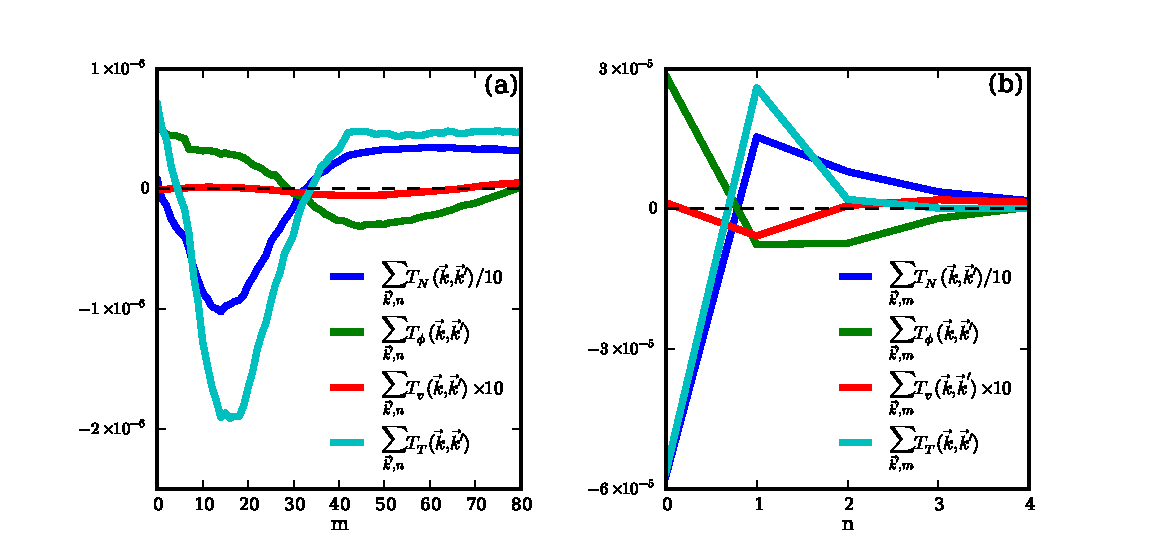
\includegraphics[]{nl_dynamics}}
\caption{Periodic simulation three-wave transfer dynamics}
\label{nl_dynamics}
\end{figure}

Fig.~\ref{mn_dynamics} only shows the dynamical pieces due to the linear terms of Eqs.~\ref{ni_eq}-~\ref{te_eq}, and they therefore don't show the nonlinear transfer between different $\vec{k}$.
The advective nonlinearities provide this transfer (the $T_j(\vec{k},\vec{k'})$ terms), 
and they are essentially conservative, meaning they provide no net injection or dissipation with respect to the fluctuations. Now the $T_j(\vec{k},\vec{k'})$ terms are each four dimensional,
making them difficult to show. I choose to sum over some of the dimensions to show some of their aggregate properties. In Fig.~\ref{nl_dynamics} a), I sum over $\vec{k'}$ and $n$ leaving them
as only functions of $m$. Also note that I have divided $T_N(\vec{k},\vec{k'})$ by $10$ and multiplied $T_v(\vec{k},\vec{k'})$ by $10$ so that all of the $T_j$ can be shown on one plot.
Notice where $T_N$ and $T_T$ are positive and where they are negative. Negative values at a particular $m$ indicate that the fluctuations with azimuthal wavenumber $m$ are giving up net energy, 
while positive values correspond to fluctuations that are taking up net energy at that $m$. 
$T_N$ and $T_T$ transfer, on the aggregate, energy in the range $5 < m < 30$ to energy at all other values of $m$. This is not at all surprising because $Q_N$ and $Q_T$ are largest
for $5 < m < 30$. This means that energy is injected from the equilibrium gradients at $5 < m < 30$ and then three-wave transferred into other azimuthal wave numbers in both forward and inverse
cascades (mostly forward). 
Actually the summation I use hides the information regarding the locality of wavenumber transfer, so it's indeterminate from this figure whether the transfer process is by cascading or non-local transfer.
I defer this detail to future work. 
On the other hand, $T_\phi$ and $T_v$ have the opposite character of $T_N$ and $T_T$, meaning that the transfer dynamics are the other way around. This is typical in 
similar systems, such as Hasegawa-Wakatani systems~\cite{hasegawa1983,Camargo1995} in which the density potential energy exhibits a forward cascade, while the perpendicular kinetic energy
exhibits an inverse cascade. It was also obvious that this had to happen given the azimuthal assymetry between $C_\phi$ and $D_\phi$ (see Fig.~\ref{mn_dynamics} c)).

More importantly, however, Fig.~\ref{nl_dynamics} b) shows the axial wavenumber transfers. Again $T_N$ and $T_T$ are similar. Both show energy transfer from $n=0$ to $n \ne 0$. This is truly important!
It is the most direct evidence for the nonlinear instability.
Our paradigmatic hypothesis in Ref.~\cite{Umansky2011} posited the opposite transfer direction. The most unstable linear eigenmodes have $n = \pm 1$ and all eigenmodes with $n=0$ are stable,
yet Fig.~\ref{nl_dynamics} b) shows that the dominant energy transfer is from $n=0$ to $n \ne 0$, at least for $N$ and $T_e$. Again, $T_\phi$ and $T_v$ have the opposite character of $T_N$ and $T_T$,
as really they must, since $\phi$ and $\vpe$ gain their energy through the adiabatic response.

\begin{figure}[!ht]
\centerline{\includegraphics[width=\textwidth]{per_en_flow_diagram}}
\caption{Periodic simulation energy flow diagram}
\label{per_en_flow_diagram}
\end{figure}

It's still difficult to see the energy flow paths from Figs.~\ref{mn_dynamics} and~\ref{nl_dynamics} alone. So I have put the results in a flow diagram -- Fig.~\ref{per_en_flow_diagram}. In order to
do this, I've summed all quantities over $m$ and $n$ (including $|n| \ge 2$), 
except that I have left $n=0$ components out of the sums and shown them separately. For instance, $Q_N(0)$ represents the density fluctuation
energy injection at $n=0$, while $Q_N(!0)$ represents the density fluctuation energy injection for all $n \ne 0$ summed together. Furthermore, the symbol $N(0)$ represents 
$\sum_{m}E_N(m,n=0)$,
$N(!0)$ represents $\sum_{m,n \ne 0} E_N(\vec{k})$, etc. Note that every term is summed over $m$.

The diagram starts at the top with the equilibrium density
and temperature profile gradients. They ultimately supply free energy for the fluctuations. Pointing out of them, the yellow $Q_j$'s extract that energy, channeling it
to the density and potential fluctuations. The $Q_j$'s
are normalized so that they sum to 100 so that each one represents a percentage of energy brought into the system. Clearly, the $n=0$ components dominate the energy injection from the equilibrium
gradients, and the density injection is much stronger than the temperature injection. The blue $T_N$ and $T_T$ three-wave transfers both go in the direction of $n=0$ to $n \ne 0$. Dissipation occurs
for every fluctuation component and takes all of the injected energy out of the system during the quasi-steady-state stage. 
Next, the red $C_N$ and $C_T$ transfer channels transfer energy from $N$ and $T_e$ to $\vpe$, only at $n \ne 0$, which is the start of the adiabatic response. Actually,
$C_T = 0$ because the parallel heat conduction is such a large dissipative factor. Completing the adiabatic response, $C_\phi$ transfers energy from $\vpe$ to $\phi$ at $n \ne 0$. Finally,
$T_\phi$ shows axial transfer into $n=0$ $\phi$ components.


\subsection{Nonlinear Instability}
\label{ss_nl_inst}

Fig.~\ref{per_en_flow_diagram} provides a look at the way energy flows through the system. The nonlinear instability mechanism can be extracted from a subset of the steps in the flow diagram.
I provide a reduced diagram in Fig.~\ref{reduced_nl_diagram} to isolate the essential interactions of the nonlinear instability mechanism. Notice that I focus only on the density fluctuation
side (as opposed to the temperature fluctuation side) because it's clear from the numbers in Fig.~\ref{per_en_flow_diagram} that the density fluctuations are a much stronger drive for
the system than the temperature fluctuations. Again, starting at the top, the $n=0$ potential fluctuations draw energy from the equilibrium density gradient by advection, depositing that
energy into the $n=0$ density fluctuations. Then, those density fluctuations nonlinearly transfer energy into $n \ne 0$ density fluctuations. Next, the adiabatic response acts to transfer
some of that energy into $n \ne 0$ potential fluctuations, which finally nonlinearly transfer energy into the $n=0$ potential fluctuations.

\begin{figure}[!ht]
\centerline{\includegraphics[]{reduced_nl_diagram}}
\caption{Nonlinear instability diagram}
\label{reduced_nl_diagram}
\end{figure}

Shown in this way, it's clear that the process is self-sustaining. It's also the dominant process by which the fluctuations get their energy from the equilibrium gradients, which is clear
from the fact that $Q_N(n=0)$ comprises $71 \%$ of all of the energy injection. Also, the net direction of $T_N$ (from $n=0$ to $n \ne 0$) and its large magnitude support this.
 
To me at least, this came as a big surprise due to my understanding of the unstable linear eigenmode drive paradigm.
Given this paradigm, it seems counterintuitive that energy can be injected into the fluctuations at $n=0$, where only
stable linear eigenmodes reside. Furthermore, linear eigenmodes are multi-field objects which have definite phase and magnitude relationships between the different fields. When there are no
nonlinearities, the entire eigenmode grows at one particular growth rate, so all of the fields must grow together. The energy dynamics analysis above seems to indicate that the fields
don't all grow together or transfer their energy in the same spectral direction.

The reason why regions in wavenumber space where only stable linear eigenmodes exist can actually inject energy into the system is that the 
linear eigenmodes are nonorthogonal and the nonlinearities can mix the nonorthogonal eigenmodes in complex ways. 
I don't show the mathematics here, but others have pointed this out and shown it before~\cite{camargo1998,kim2010}. The implication is that stable linear eigenmodes, 
taken in concert with one another, can inject energy into a system and mix so that the different individual fields act in different ways.
Nonorthogonal bases can produce results that are just too complicated to be of use.
For these reasons, I abandoned the linear eigenmode decomposition approach early on and chose the simpler decomposition detailed in Chapter~\ref{c_en_formalism}. 
Notice that my decomposition actually takes each field separately. I do not attempt
to create composit objects of different fields, like others have done using 
linear eigenvectors~\cite{baver2002,terry2002,terry2006a,terry2006b,gatto2006,terry2009,kim2010,makwana2011}. This choice reflects
the fact that the different fields can act in different ways.

Now, after I found this curious nonlinear instability, I wondered if others had previously found this. After all, the equations and the geometry that I use are not new. In fact, a look at 
Fig.~\ref{reduced_nl_diagram} reveals that even simpler models like the 3D Hasegawa-Wakatani equations~\cite{hasegawa1983} contain the proper components to cause the nonlinear instability. And 
cylindrical simulations of the Hasegawa-Wakatani equations are three decades old (although the original simulations were 2D).
My search of the literature reveals that this nonlinear instability was, in fact, identified in 1995. Actually, going even further back, in 1977-1979, 
Cheng et al.~\cite{cheng1977,cheng1979} performed 3D turbulence simulations that may have actually been driven by the nonlinear instability. 
In their work, they identified a dominance of $k_\para=0$ ``convective cells [that] are non-linearly excited as a result of mode-coupling of the drift instabilities.'' 
It's unclear what equation set they used
and what exactly they meant by this mode coupling, but their results seem similar to mine, and it's reasonable to believe that they at least identified the consequences of the nonlinear instability.

In 1995, Biskamp and Zeiler simulated local cylindrical plasma fluid turbulence in the first published use of the 3D Hasegawa-Wakatani equations~\cite{biskamp1995}. 
Using an energetics analysis, they in fact, correctly identified the nonlinear instability mechanism that drove the $k_\para=0$ structures in their simulations. So the nonlinear instability
mechanism is, in fact, not new. Furthermore, others expanded on this original work. 
Drake et al. showed that elimination of the linear instability by removing the $k_\para \ne 0$ components of the linear drive term
had virtually no affect on the turbulence~\cite{drake1995}. Furthermore, they showed that adding magnetic shear, which also stabilized the linear drift waves, did not stop the turbulence
from sustaining itself. Both of these showed that the nonlinear instability could act as a subcritical instability.
Additionally, B.D. Scott and others have explore nonlinear drift wave turbulence in a number of different models with different physics effects such as magnetic shear and curvature
and found that drift wave turbulence with very long parallel structures tends to sustain itself despite the presence or lack thereof of linear 
instabilities~\cite{scott1990,scott1992,zeiler1996,zeiler1997,korsholm1999,scott2002,scott2003,scott2005}.

Nevertheless, it still seems as though no one showed that nonlinear-instability driven drift wave turbulence was relevant to an experiment and not just a simulation artifact. I have attempted
to do this here and in published papers~\cite{friedman2012b,friedman2013},
showing that the simulations driven by the nonlinear instability are validated against experiment (see Sec.~\ref{s_stat_exam}). Also, I will show next that the nonlinear instability
is crucial for the simulation to produce experimentally-consistent turbulence.


\section{n=0 Suppression}
\label{s_n0_supp}

I previously introduced the $n=0$ suppressed simulation in Sec.~\ref{s_stat_exam}, where I discussed the nature of the simulation and some of its statistical properties. I claimed before that
this simulation, in which I artificially remove the $n=0$ components of the density, temperature, and potential fluctuations, eliminates the nonlinear instability.
The details of the nonlinear instability mechanism described in the previous section should now make it obvious why removing these components eliminates the nonlinear instability.
One may also consider other ways to remove the nonlinear instability while keeping the linear drift wave instability intact. For example, one could remove the $n=0$ component of the linear
drive terms or remove one or more of the nonlinear advection terms, although this would affect quite a bit more than just the nonlinear instability. In any case, my method
certainly removes the nonlinear instability mechanism while keeping the linear instability intact, allowing the simulation to act more in the paradigmatic manner.

Rather than showing another diagram of the energy flow for the $n=0$ suppressed simulation, I present the energy dynamics data in a new, compressed way. That is, I construct a growth rate
spectrum from the energy dynamics. I define the growth rate as:

\beq
\label{gamma_def}
\gamma(\vec{k}) = \pdiff{E_{tot}({\vec{k}})}{t} \bigg|_{lin} \bigg/ \left( 2 E_{tot}(\vec{k}) \right) = \sum_j \left[ Q_j(\vec{k}) + D_j(\vec{k}) \right] \bigg/ \left( 2 E_{tot}(\vec{k}) \right).
\eeq

Recall that $\sum_j C_j(\vec{k}) = 0$, so $C_j$ does not appear in this sum. I also only include the linear contribution to $ \pdiff{E_{tot}({\vec{k}})}{t}$ so that the growth rate
only involves the energy injection and dissipation at each wavenumber and not the three-wave transfers ($T_j(\vec{k},\vec{k'})$). 
Adding the three-wave transfers would always make this sum about equal to zero in the turbulent
quasi-steady state stage of the simulation anyway, rendering this quantity useless. 
In the linear stage of the simulations, this method reproduces the linear growth rate spectrum.
Specifically, this $\gamma$ is equivalent to the linear growth rate for the fastest growing branch $n=1$ eigenmodes.
I actually used this $\gamma$ to generate the curves in Figs.~\ref{lin_dw_gamma} and~\ref{lin_all_gamma}, though I used other methods to confirm the accuracy of this calculation.
$\gamma$ can also be applied to the turbulent stage of the simulation, in which it gives a composit look at the net energy injection into the system at each $\vec{k}$ normalized
by the steady-state energy at that given $\vec{k}$.

\begin{figure}[!ht]
\centerline{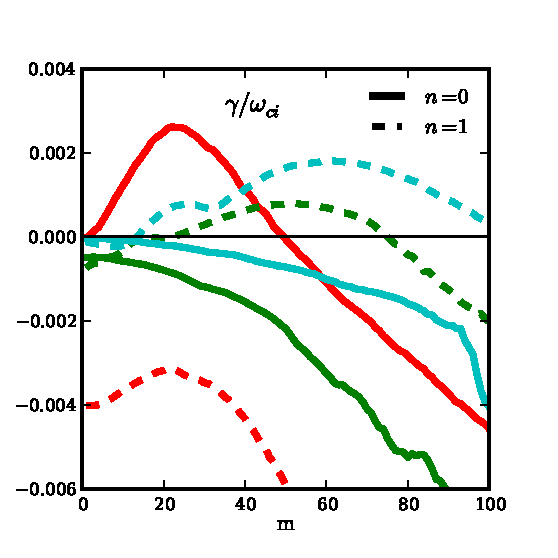
\includegraphics[]{lin_per_non0_gamma}}
\caption{Linear vs. nonlinear growth rates}
\label{lin_per_non0_gamma}
\end{figure}

Fig.~\ref{lin_per_non0_gamma} shows the results of this calculation for three different cases. First, the light blue (cyan) curves represent $\gamma(m)$ for $n=1$ (the solid line)
and $n=0$ (the dashed line) for the Periodic simulation during the linear exponential growth stage. The $n=1$ curve is the same as that shown in Figs.~\ref{lin_dw_gamma} and~\ref{lin_all_gamma}.
The $n=0$ curve, on the other hand, is the linear growth rate of the $n=0$ linear eigenmodes, which all have negative growth rates of course. The red curves map out $\gamma$ for the 
turbulent stage of the Periodic simulation. The $n=0$ growth rate is \emph{positive} for low $m$, while the $n=1$ growth rate is negative for all $m$. This isn't surprising given the
previous section's evidence for $n=0$ energy injection due to the nonlinear instability, but it is certainly a nice way to show the contrast with the linear growth rate curves.
Finally, the green curves are the growth rates for the $n=0$ suppressed simulation during the ``turbulent phase'' (recall from Fig.~\ref{n_statistics} that the fluctuations remain rather
coherent, and the state is only weakly turbulent). 
These growth rates are somewhat similar to the linear growth rates, representative of the expectation under the unstable linear eigenmode paradigm. 

Now, one may wonder why there is any $n=0$ growth rate curve at all for the $n=0$ suppressed simulation. 
The reason is because I remove the $n=0$ components after they are nonlinearly excited. I allow the nonlinearities to transfer energy 
into the $n=0$ components at each time step and then I save the data. The energy, by the way, is transferred from $n=1$ to $n=0$ modes as in the paradigmatic process. Then, I remove
these $n=0$ components before the equations are evolved again. So there are small values for these $n=0$ components that come out in the data, but are not used to evolve the equations. This allows
construction of the $n=0$ growth rate curve.
Furthermore, notice that the $n=0$ suppressed simulation growth rates do not exactly match the linear growth rates. The reason for this is that the nonlinearities change the structures and
phases between the fields. Or to put it another way, they excite slower growing or damped eigenmodes that lessen the effect of the most unstable eigenmodes. This is consistent with the linear
instability paradigm.

\begin{figure}[!ht]
\centerline{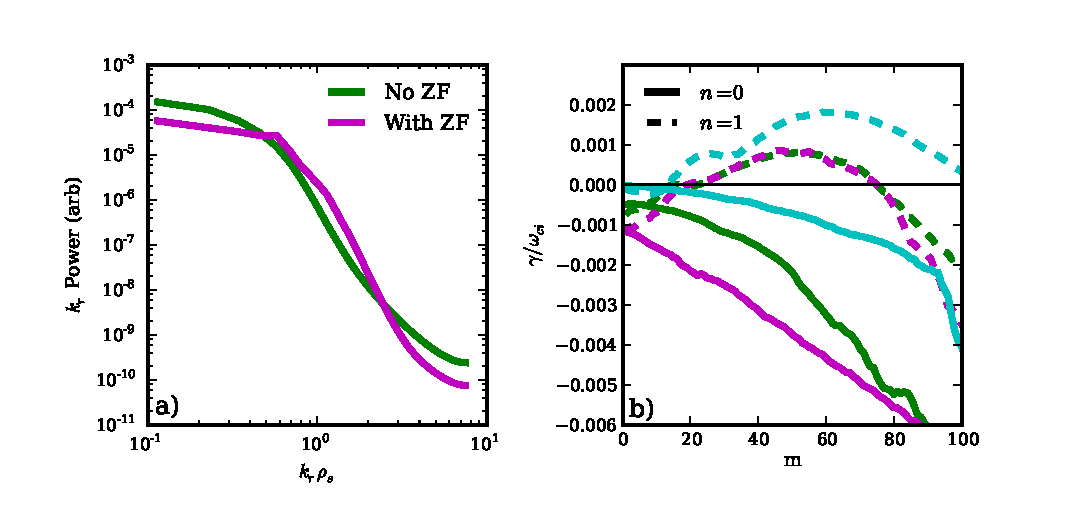
\includegraphics[]{zf_gamma_spec}}
\caption{Zonal flow affect on spectra and growth rate}
\label{zf_gamma_spec}
\end{figure}

Finally, one might notice that manually removing all of the $n=0$ fluctuation components means that the zonal flows ($n=0, m=0$ component of $\phi$) are also removed. 
Zonal flows are often seen as being an important saturation mechanism for turbulence by either shearing the turbulent eddies~\cite{biglari1990} or by exciting stable eigenmodes~\cite{makwana2012}.
They are often considered to provide the most important nonlinear interactions to plasma turbulence. So one might naively think that their removal in the $n=0$ suppressed simulation
causes the removal of the nonlinear instability. I say ``naively'' because the nonlinear instability mechanism outlined in Fig.~\ref{reduced_nl_diagram} doesn't depend upon zonal flows.
But to prove this and to explore the real affect of the zonal flows, I have rerun the $n=0$ suppressed simulation without removing the zonal flows. I still remove all of the $n=0$
components of the density and temperature fluctuations and all of the $n=0, m \ne 0$ components of $\phi$, but I leave the zonal flow component intact. I show some comparisons of the two
simulations in Fig.~\ref{zf_gamma_spec}. In Fig.~\ref{zf_gamma_spec} a), I show the $k_r$ spectrum of the two simulations, revealing that the zonal flows cause radial wavenumber transfers
from low $k_r$ to medium $k_r$. This is a simple consequence of a three-wave interaction between the dominant low $k_r$ structures and the zonal flows which have finite $k_r$. This interaction
causes a slight saturation effect because the medium $k_r$ modes have lower growth rates than the low $k_r$ modes, and the overall saturation level is depressed by about a factor of 2
when I retain the zonal flows.

Nevertheless, the zonal flows don't cause the nonlinear instability, which is evident from Fig.~\ref{zf_gamma_spec} b) where the nonlinear growth rates of the two simulations are shown
along with the linear growth rates. Recall from Fig.~\ref{lin_per_non0_gamma} how different the growth rates look when the nonlinear instability is present.
The simulation with the zonal flows is qualitatively similar to the simulation without the zonal flows, but as expected, the growth rates with the zonal flows are less than or equal to
the growth rates without the zonal flows. Interestingly, the zonal flows only affect the growth rates at $n=1$ at very low and very high $m$, but they affect the $n=0$ growth rates
mostly at medium $m$. Anyhow, the zonal flows don't affect the nonlinear instability, and they also have a relatively weak affect on turbulent saturation compared to some other types
of turbulence like ITG turbulence~\cite{dimits2000,Holland2003}.

